\documentclass[spanish, fleqn]{article}
\usepackage{babel}
\usepackage[utf8]{inputenc}
\usepackage{amsmath}
\usepackage{amsfonts}
\usepackage[colorlinks, urlcolor=blue]{hyperref}
\usepackage{fourier}
\usepackage{tikz}
\usepackage[top = 2.5cm, bottom = 2cm, left = 2cm, right = 2cm]{geometry}

\usetikzlibrary{automata, arrows, positioning, babel}
\tikzset{shorten >= 1pt,
	 node distance = 1.8cm, on grid,
	 >= stealth,
	 initial text = Inicio,
	 every state/.style = {draw, very thick,
			       minimum size = 5mm},
	 bend angle = 35,
	 every loop/.style = {looseness = 13}}

\newcommand{\num}{1}

\title{Informática Teórica\\
       Tarea \#\num \\
       ``Esto no se compila''}
\author{Andrés Navarro // 201673001-K}
\date{25 de septiembre de 2017}

\begin{document}
\maketitle
\pagestyle{empty}
\thispagestyle{empty}

  Una forma alternativa de construir una expresión regular
  que reconoce el lenguaje aceptado
  por el DFA \(M = (Q, \Sigma, \delta, q_0, F)\)
  es plantear expresiones regulares
  para las palabras que llevan al DFA desde el estado inicial
  a cada uno de los estados.
  Básicamente,
  llamando \(R_q\) a la expresión para llegar al estado \(q\),
  si \(\delta(q, a) = p\),
  entre las alternativas para \(R_p\) estará \(R_q a\).
  El lenguaje aceptado por \(M\) es la alternancia entre las expresiones
  para estados finales.

  Esto termina en un sistema de ecuaciones para los distintos \(R_q\),
  podemos usar nuestro teorema
  sobre solución de ecuaciones de la forma \(X = X A \cup B\) entre lenguajes
  para resolver una de ellas,
  y substituir en las demás,
  hasta finalmente tener todos los \(R_q\) requeridos.

  Comentarios en C++ quedan definidos
  por el DFA de la figura~\ref{fig:20172t2},
  donde hemos omitido el estado muerto
  y las transiciones a él para simplificar.
  El alfabeto usado es \(\{ /, *, a, n \}\),
  donde \(/\) y \(*\) representan esos caracteres,
  \(n\) representa al fin de línea
  (se escribe \('\backslash n'\) en C++)
  y \(a\) es cualquier otro caracter válido.
  \begin{figure}[ht]
    \centering
    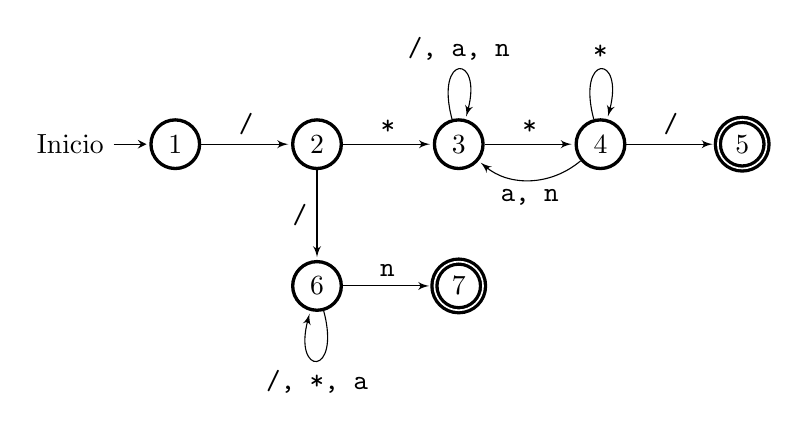
\begin{tikzpicture}
      \node [initial, state] (1) {1};
      \node [state] (2) [right of = 1] {2};
      \node [state] (3) [right of = 2] {3};
      \node [state] (4) [right of = 3] {4};
      \node [state, accepting] (5) [right of = 4] {5};
      \node [state] (6) [below of = 2] {6};
      \node [state, accepting] (7) [right of = 6] {7};
      \path[-latex'] (1) edge [above] node {\texttt{/}} (2)
		     (2) edge [above] node {\texttt{*}} (3)
		     (2) edge [left]  node {\texttt{/}} (6)
		     (3) edge [above] node {\texttt{*}} (4)
		     (4) edge [above] node {\texttt{/}} (5);
      \path[-latex'] (3) edge [loop above] node {\texttt{/, a, n}} ()
		     (4) edge [loop above] node {\texttt{*}} ();
      \path[-latex'] (4) edge [bend left = 40] node[below]
				 {\texttt{a, n}} (3);
      \path[-latex'] (6) edge [loop below] node {\texttt{/, *, a}} ()
		     (6) edge [above] node {\texttt{n}} (7);
    \end{tikzpicture}
    \caption{Comentarios en C++}
    \label{fig:20172t2}
  \end{figure}
  \begin{enumerate}
  \item % 20172t2p1
    Plantee el sistema de ecuaciones descrito
    para expresiones regulares \(R_1\) a \(R_7\)
    partiendo del autómata de la figura~\ref{fig:20172t2}.
    Use \(s\) en vez del símbolo \(*\) para evitar ambigüedades.
    
    Dado que $R_{1}$ es el correspondiente al estado $1$, el cual es el inicial, se llega a el consumiendo solamente $\epsilon$, para el resto de expresiones $R_{n}$, su ecuación fue confecionada visualizando el autómata. 
    \begin{align*}
    &R_{1}=\epsilon \\
    &\text{A $R_2$ solo se puede llegar desde $R_1$ consumiendo /.}\\
    &R_{2}=R_{1}/\\
    &\text{Para $R_3$ podemos llegar desde $R_2$ consumiendo s, desde el mismo consumiendo a,n o /, o}\\
    &\text{desde $R_4$ consumiendo a o n.}\\
    &R_{3}=R_{2}s|R_{3}/|R_{3}a|R_{3}n|R_{4}a|R_{4}n\\
    &\text{A $R_4$ se puede llegar desde $R_3$ consumiendo s, o desde el mismo consumiendo s.}\\
    &R_{4}=R_{3}s|R_{4}s
    \end{align*}
    \begin{align*}
    &\text{Para $R_5$ se tiene que solo se puede llegar desde $R_4$ consumiendo /.}\\
    &R_{5}=R_{4}/\\
    &\text{Para $R_6$ se puede llegar consumiendo / desde $R_2$ o desde el mismo consumiendo s o a.}\\
    &R_{6}=R_{2}/|R_{6}/|R{6}s|R_{6}a\\
    &\text{Por último, para $R_7$ se tiene que se puede llegar a el desde $R_6$ consumiendo n.}\\
    &R_{7}=R_{6}n
    \end{align*}
    Finalmente tenemos el sistema:
    \begin{align*}
    R_{1}&=\epsilon \\
    R_{2}&=R_{1}/\\
    R_{3}&=R_{2}s|R_{3}/|R_{3}a|R_{3}n|R_{4}a|R_{4}n\\
    R_{4}&=R_{3}s|R_{4}s\\
    R_{5}&=R_{4}/\\
    R_{6}&=R_{2}/|R_{6}/|R{6}s|R_{6}a\\
    R_{7}&=R_{6}n\\
	\end{align*}
  \item % 20172t2p2
    \label{ques:20172t2p2}
    Dé la expresión regular para el lenguaje aceptado por el autómata
    en términos de los \(R_k\).
    
    Se trabajará sobre las ecuaciones.
    \begin{align*}
    &\text{Tanto $R_1$ como $R_2$ permanecen igual.}\\
    &R_{1}=\epsilon \\
    &R_{2}=R_{1}/\\
    &\text{Reemplazando $R_2$ en $R_3$.}\\
    &R_{3}=R_{2}s|R_{3}/|R_{3}a|R_{3}n|R_{4}a|R_{4}n \Rightarrow  R_{3}=R_{1}/s|R_{3}/|R_{3}a|R_{3}n|R_{4}a|R_{4}n\\
    &\text{Ahora, en $R_4$ reemplazamos $R_3$.}\\
    &R_4=R_{3}s|R_{4}s \Rightarrow R_4=(R_{1}/s|R_{3}/|R_{3}a|R_{3}n|R_{4}a|R_{4}n)s|R_4s\\
    &\text{En $R_5$ finalmente nos queda:}\\
    &R_{5}=((R_{1}/s|R_{3}/|R_{3}a|R_{3}n|R_{4}a|R_{4}n)s|R_4s)/\\
    &\text{Por otro lado, reemplazando $R_2$ en $R_6$:}\\
    &R_6=R_{2}/|R_{6}/|R{6}s|R_{6}a \Rightarrow R_6=R_{1}//|R_{6}/|R{6}s|R_{6}a\\
    &\text{Finalmente $R_7$ queda como:}\\
    &R_7=R_6n \Rightarrow R_7=(R_{1}//|R_{6}/|R{6}s|R_{6}a)n\\
    \end{align*}    
    Dado que nuestro DFA tiene dos estados finales, nuestra expresion regular estará dada por los $R_n$ correspondientes a estos
    dos estados. Estos estados corresponden al 5 y al 7, por lo que nuesto RE sería:
    \begin{align*}
	&RE=R_5 | R_7\\
    &\text{Si reemplazamos con lo obtenido:}\\
    &RE=((R_{1}/s|R_{3}/|R_{3}a|R_{3}n|R_{4}a|R_{4}n)s|R_4s)/|(R_{1}//|R_{6}/|R{6}s|R_{6}a)n
    \end{align*}
        
  \item % 20172p2t3
    Indique paso a paso cómo resuelve el sistema de ecuaciones
    para las variables necesarias para la pregunta~\ref{ques:20172t2p2}.
	
	Recordar que el teorema 1.1 nos dice que:
	\begin{align*}
	&X = A | XB \Rightarrow X = AB^*\\
	&\text{O bien:}\\
	&X = A | BX \Rightarrow X = B^*A
	\end{align*}	    
    
    Primero reemplazamos $R_{1}$ en $R_{2}$
    \begin{align*}
    R_{1}&=\epsilon \\
    R_{2}&=R_{1}/ \Rightarrow R_{2}=\epsilon/ \Rightarrow R_{2}=/
    \end{align*}
    Trabajando sobre $R_3$
    \begin{align*}
    &\text{Primero tenemos:}\\
    &R_3=R_{4}a|R_{4}n \Rightarrow R_3=R_4(a|n)\\
    &\text{Con lo obtenido anteriormente de $R_2$:}\\
    &R_3=R_2s \Rightarrow R_3=/s\\
    &\text{Tenemos:}\\
    &R_3=/s|R_{3}/|R_{3}a|R_{3}n|R_4(a|n) \Rightarrow R_3=/s|R_3(/|a|n)|R_4(a|n) \\
    &\text{Ahora, ocupando el teorema 1.1:}\\
    &R_3=/s|R_3(/|a|n) \Rightarrow R_3=/s(/|a|n)^*\\
    &R_3=R_4(a|n)|R_3(/|n|a) \Rightarrow R_3=R_4(a|n)(/|n|a)^*\\
    &\text{Finalmente:}\\
    &R_3=/s(/|a|n)^*|R_4(a|n)(/|n|a)^*
    \end{align*}
    Trabajando sobre $R_4$
    \begin{align*}
    &\text{Ocupando el teorema 1.1 tenemos:}\\
    &R_4=R_3s|R_4s \Rightarrow R_4=R_3ss^*\\
    &\text{Sabiendo que $ss*=s^+$:}\\
    &R_4=R_3s^+\\
    &\text{Con lo obtenido en $R_3$:}\\
    &R_4=(/s(/|a|n)^*|R_4(a|n)(/|n|a)^*)s^+ \Rightarrow R_4=/s(/|a|n)^*s^+|R_4(a|n)(/|n|a)^*s^+\\
    &\text{Ocupando el teorema 1.1 tenemos:}\\
    &R_4=/s(/|a|n)^*s^+|R_4(a|n)(/|n|a)^*s^+ \Rightarrow R_4=/s(/|a|n)^*s^+((a|n)(/|n|a)^*s^+)^*
    \end{align*}
    Trabajando sobre $R_5$
    \begin{align*}
	&\text{Ocupando lo obtenido en $R_4$:}\\
    &R_5=R_4/ \Rightarrow R_5=/s(/|a|n)^*s^+((a|n)(/|n|a)^*s^+)^*/
    \end{align*}
    Trabajando sobre $R_6$:
    \begin{align*}
	&R_6=R_{6}/|R_{6}s|R_{6}a \Rightarrow R_6=R_6(/|s|a)\\
	&\text{Ocupando el teorema 1.1 tenemos:}\\
	&R_6=R_2/|R_6(/|s|a) \Rightarrow R_6=R_2/(/|s|a)^*\\
	&\text{Reemplazando $R_2$:}\\
	&R_6=//(/|s|a)^*
    \end{align*}
    Trabajando sobre $R_7$:
    \begin{align*}
    &\text{Reemplazando $R_6$:}\\
    &R_7=R_6n \Rightarrow R_7=//(/|s|a)^*n
    \end{align*}
    
    Con lo respondido en la pregunta 2, sabemos que la RE esta descrita por:
    \begin{align*}
    &RE=R_5|R_7\\
    &\text{Reemplazando con lo obtenido:}\\
    &RE=/s(/|a|n)^*s^+((a|n)(/|n|a)^*s^+)^*/|//(/|s|a)^*n
    \end{align*}
  \end{enumerate}
\end{document}

%%% Local Variables:
%%% mode: latex
%%% TeX-master: t
%%% End:
